\documentclass{article}
\usepackage{arxiv}

\usepackage[utf8]{inputenc}
\usepackage[english]{babel}
\usepackage[T1]{fontenc}
\usepackage{url}
\usepackage{booktabs}
\usepackage{amsfonts}
\usepackage{nicefrac}
\usepackage{microtype}
\usepackage{lipsum}
\usepackage{graphicx}
%\usepackage{natbib}
\usepackage{doi}



\title{Image Style Transfer for Distillation of Diffusion Knowledge into a Transformer}

\author{ Egor Y.~Silvestrov \\
	Faculty of Computational Mathematics and Cybernetics \\
	Lomonosov Moscow State University \\
	Moscow, Russia \\
	\texttt{s02210546@gse.cs.msu.ru} \\
	%% examples of more authors
	\And
        Victor V.~Kitov \\
	Faculty of Computational Mathematics and Cybernetics \\
	Lomonosov Moscow State University \\
	Moscow, Russia \\
	\texttt{v.v.kitov@yandex.ru} \\
	%% \AND
	%% Coauthor \\
	%% Affiliation \\
	%% Address \\
	%% \texttt{email} \\
	%% \And
	%% Coauthor \\
	%% Affiliation \\
	%% Address \\
	%% \texttt{email} \\
	%% \And
	%% Coauthor \\
	%% Affiliation \\
	%% Address \\
	%% \texttt{email} \\
}
\date{}

\renewcommand{\shorttitle}{\textit{arXiv} Template}

%%% Add PDF metadata to help others organize their library
%%% Once the PDF is generated, you can check the metadata with
%%% $ pdfinfo template.pdf
\hypersetup{
pdftitle={A template for the arxiv style},
pdfsubject={q-bio.NC, q-bio.QM},
pdfauthor={Egor Y.~Silvestrov, Victor V.~Kitov},
pdfkeywords={},
}

\begin{document}
\maketitle

\begin{abstract}
	Modern methods of style transfer for weak models often face problems with the quality of style transfer, especially in conditions of limited computing resources and untagged data (unsupervised learning). Distilling knowledge through diffusion models is a promising approach to improve the quality of weak models by transferring key elements of knowledge from more powerful models by creating a marked-up dataset and turning an unsupervised task into a supervised task with a teacher. In this paper, we investigate the method of distilling knowledge for a diffusion model, which allows us to adapt the styling and transmission of content for a more lightweight model (based on the transformer architecture) without the need for significant computational costs. As a result, an optimal balance is achieved between maintaining high-quality visual characteristics and cost-effectiveness, which opens up new opportunities for developing effective stylization models in real time.
\end{abstract}


\keywords{Image Style Transfer \and Diffusion Model \and Knowledge Distillation \and Transformer}

\section{Introduction}
    Image style transfer has gained significant attention in the creation of artistic visuals. The task involves taking a content image and a style reference image to produce an output that retains core content elements while adopting the visual style of the reference. This technique has applications across various domains, such as clothing design \cite{method 6}, photo and video editing \cite{method 7, method 8}, virtual reality \cite{method 9}, and more. Recently, deep neural networks have been widely used for style transfer, which can be grouped into three main approaches: 1) optimization-based methods, 2) feedforward approximation, and 3) zero-shot style transfer. Gates et al. \cite{method 10} proposed optimizing pixel values in a content image by minimizing both feature reconstruction and style losses, producing impressive results but requiring multiple iterations for each content-style pair, making it computationally expensive. In response, feedforward networks \cite{method 11, method 12, method 13} were developed to directly learn mappings from photographs to stylized images in specific painting styles, although retraining is required for new styles. Zero-shot style transfer is more versatile, as it can handle diverse styles, even previously unseen ones. Huang et al. \cite{method 14} introduced an arbitrary style transfer approach using adaptive instance normalization (AdaIN), which normalizes content image features and adjusts them based on style parameters. Recent work replaces AdaIN with whitening and coloring transformations \cite{method 15}, while several studies further refine this approach \cite{method 16, method 17}.
    
    However, a common limitation of these methods is that merely adjusting feature statistics makes it difficult to synthesize complex style patterns rich in detail and local structures, often resulting in distorted and less recognizable images. For instance, methods by Gatys et al. \cite{method 10}, AdaIN \cite{method 14}, and WCT \cite{method 15} frequently introduce style distortions that blur original content details. To address this, Deng et al. developed StyTr2 \cite{method 18}, which uses attention to capture semantic correlations between content and style features, yielding visually appealing results. Nevertheless, StyTr2 also suffers from structure distortion due to its shallow feature extractor, which lacks pre-trained weights, limiting its ability to differentiate between foreground and background objects. Thus, achieving a representation that can maintain content structure while accurately capturing fine-grained style patterns remains a challenging problem.
    
    Diffusion models \cite{method 1, method 2, method 3, method 4} have also achieved remarkable success in style transfer, excelling at generating visually coherent and detailed stylizations. In this paper, we propose using STTR \cite{method 5}, a Transformer-based model, as a student model to distill knowledge from a larger diffusion model \cite{method 4}. This diffusion model was taken based on good experimental results and the existence of an implementation. In this setup, the diffusion model \cite{method 4} performs style transfer on images, and STTR \cite{method 5} is trained to replicate these stylized outputs, effectively reframing style transfer as a supervised learning task. Transformer-based architectures, popularized by advancements in natural language processing \cite{method 19}, have demonstrated effectiveness in vision tasks by modeling long-range dependencies. The STTR \cite{method 5} approach uses to decompose content and style images into visual tokens, enabling learning of the global context between them. As similar content tokens align with the corresponding style tokens, this approach achieves detailed style transformation with structural consistency between content and style.

    We believe that training a small, relatively diffusive transformer model will allow us to achieve the quality of large diffusive models while using much fewer resources, which allows us to run this model on various low-power devices.

\section{Related work}
\label{sec:headings}

\subsection{Diffusion Model-based Neural Style Transfer}
\lipsum[5]

\lipsum[4] See Section \ref{sec:headings}.

\section{Method}
\label{sec:headings}


\subsection{Architecture}
\lipsum[5]
\begin{equation}
	\xi _{ij}(t)=P(x_{t}=i,x_{t+1}=j|y,v,w;\theta)= {\frac {\alpha _{i}(t)a^{w_t}_{ij}\beta _{j}(t+1)b^{v_{t+1}}_{j}(y_{t+1})}{\sum _{i=1}^{N} \sum _{j=1}^{N} \alpha _{i}(t)a^{w_t}_{ij}\beta _{j}(t+1)b^{v_{t+1}}_{j}(y_{t+1})}}
\end{equation}

\subsubsection{Adapting Large-scale Diffusion Models for Style Transfer}
\lipsum[6]

\subsubsection{STyle TRansformer(STTR)}
\lipsum[6]

\paragraph{Paragraph}
\lipsum[7]

\section{Experiments}
\label{sec:experimetns}
\lipsum[7]

\section{Conclusion}
\label{sec:conclusion}
\lipsum[7]

\section{Examples of citations, figures, tables, references}
\label{sec:others}

\subsection{Citations}
Citations use \verb+natbib+. The documentation may be found at
\begin{center}
	\url{http://mirrors.ctan.org/macros/latex/contrib/natbib/natnotes.pdf}
\end{center}

Here is an example usage of the two main commands (\verb+citet+ and \verb+citep+): Some people thought a thing \citep{kour2014real, hadash2018estimate} but other people thought something else \citep{kour2014fast}. Many people have speculated that if we knew exactly why \citet{kour2014fast} thought this\dots

\subsection{Figures}
\lipsum[10]
See Figure \ref{fig:fig1}. Here is how you add footnotes. \footnote{Sample of the first footnote.}
\lipsum[11]

% \begin{figure}
% 	\centering
% 	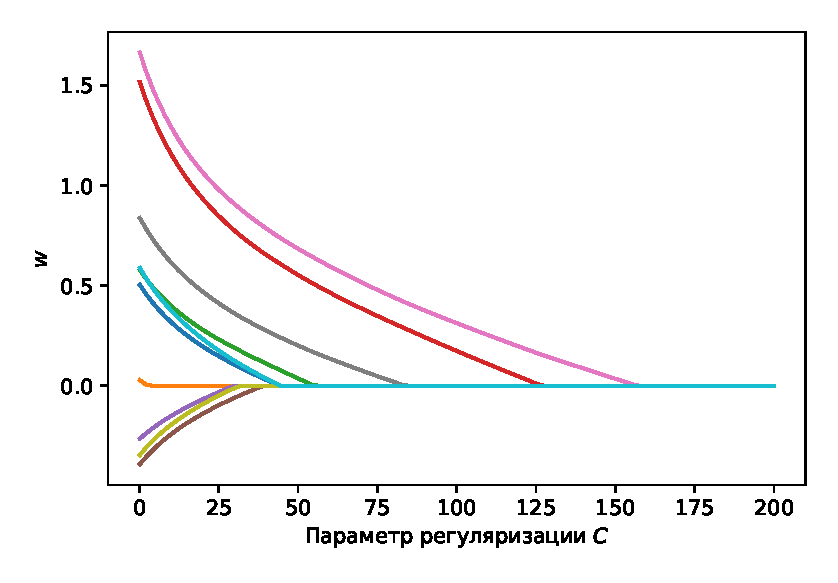
\includegraphics[width=0.5\textwidth]{../figures/log_reg_cs_exp.eps}
% 	\caption{Sample figure caption.}
% 	\label{fig:fig1}
% \end{figure}

\subsection{Tables}
See awesome Table~\ref{tab:table}.

The documentation for \verb+booktabs+ (`Publication quality tables in LaTeX') is available from:
\begin{center}
	\url{https://www.ctan.org/pkg/booktabs}
\end{center}


\begin{table}
	\caption{Sample table title}
	\centering
	\begin{tabular}{lll}
		\toprule
		\multicolumn{2}{c}{Part}                   \\
		\cmidrule(r){1-2}
		Name     & Description     & Size ($\mu$m) \\
		\midrule
		Dendrite & Input terminal  & $\sim$100     \\
		Axon     & Output terminal & $\sim$10      \\
		Soma     & Cell body       & up to $10^6$  \\
		\bottomrule
	\end{tabular}
	\label{tab:table}
\end{table}

\subsection{Lists}
\begin{itemize}
	\item Lorem ipsum dolor sit amet
	\item consectetur adipiscing elit.
	\item Aliquam dignissim blandit est, in dictum tortor gravida eget. In ac rutrum magna.
\end{itemize}


% \bibliographystyle{unsrtnat}
% \bibliography{references.bib}


\renewcommand{\bibname}{References}
\addcontentsline{toc}{section}{\bibname}

\begin{thebibliography}{9} 
    \bibitem{method 1} 
    \href{https://arxiv.org/pdf/2308.07863}{Z. Wang, L. Zhao and W. Xing, “StyleDiffusion: Controllable Disentangled Style Transfer via Diffusion Models”, College of Computer Science and Technology, Zhejiang University, 2023.}
    \bibitem{method 2} \href{https://openaccess.thecvf.com/content/CVPR2023/papers/Zhang_Inversion-Based_Style_Transfer_With_Diffusion_Models_CVPR_2023_paper.pdf}{Y. Zhang, N. Huang, F. Tang, H. Huang, C. Ma, W. Dong, C. Xu, “Inversion-based Style Transfer with Diffusion Models”, MAIS, Institute of Automation, Chinese Academy of Sciences, Institute of Computing Technology, Chinese Academy of Sciences, School of AI, UCAS, Kuaishou Technology, 2023.}
    \bibitem{method 3} \href{https://openaccess.thecvf.com/content/ICCV2023/papers/Yang_Zero-Shot_Contrastive_Loss_for_Text-Guided_Diffusion_Image_Style_Transfer_ICCV_2023_paper.pdf}{S. Yang, H. Hwang, J. Chul Ye, “Zero-Shot Contrastive Loss for Text-Guided Diffusion Image Style Transfer”, Kim Jaechul Graduate School of AI, Korea Advanced Institute of Science and Technology (KAIST), 2023.}
    \bibitem{method 4} 
    \href{https://arxiv.org/pdf/2312.09008}{J. Chung, S. Hyun, J. Heo, “Style Injection in Diffusion: A Training-free Approach
    for Adapting Large-scale Diffusion Models for Style Transfer”, Sungkyunkwan University, 2024.}
    \bibitem{method 5} 
    \href{https://arxiv.org/pdf/2210.05176v1}{J. Wang, H. Yang, J. Fu, T. Yamasaki and B. Guo, “Fine-Grained Image Style Transfer
    with Visual Transformers”,  The Univerisity of Tokyo, Microsoft Research, 2022.}
    \bibitem{method 6} 
    \href{https://arxiv.org/pdf/1707.09899}{P. Date, A. Ganesan, T. Oates, “Fashioning with Networks: Neural Style Transfer to Design
    Clothes”,  University Of Maryland, 2017.}
    \bibitem{method 7} 
    \href{https://arxiv.org/pdf/1703.09211}{D. Chen, J. Liao, L. Yuan, N. Yu and G. Hua, “Coherent Online Video Style Transfer”,  University Of Maryland, 2017.}
    \bibitem{method 8} \href{https://www.researchgate.net/publication/234096926_Style_Transfer_Via_Im  age_Component_Analysis}{W. Zhang, C. Cao, S. Chen, J. Liu, “Style Transfer Via Image Component Analysis”,  2013.}
    \bibitem{method 9} 
    \href{https://arxiv.org/pdf/1701.02357}{C. Castillo, S. De, X. Han, B. Singh, A. K. Yadav, and T. Goldstein, “Son of Zorn’s Lemma: Targeted style transfer using instance-aware semantic segmentation”, Department of Computer Science, University of Maryland, College Park, 2017.}
    \bibitem{method 10} 
    \href{https://www.cv-foundation.org/openaccess/content_cvpr_2016/papers/Gatys_Image_Style_Transfer_CVPR_2016_paper.pdf}{Leon A. Gatys, Alexander S. Ecker, Matthias Bethge, “Image Style Transfer Using Convolutional Neural Networks”, Centre for Integrative Neuroscience, University of Tubingen, 2016.}
    \bibitem{method 11} 
    \href{https://arxiv.org/pdf/1603.08155}{J. Johnson, A. Alahi, L. Fei-Fei, “Perceptual Losses for Real-Time Style Transfer and Super-Resolution”, Department of Computer Science, Stanford University, 2016.}
    \bibitem{method 12} 
    \href{https://arxiv.org/pdf/1604.04382}{C. Li and M. Wand, “Precomputed Real-Time Texture Synthesis with Markovian Generative Adversarial Networks”, Institut for Informatik, University of Mainz, 2016.}
    \bibitem{method 13} 
    \href{https://arxiv.org/pdf/1603.03417}{D. Ulyanov, V. Lebedev, A. Vedaldi, V. Lempitsky, “Texture Networks: Feed-forward Synthesis of Textures and Stylized Images”, Skolkovo Institute of Science and Technology \& Yandex, 2016.}
    \bibitem{method 14} 
    \href{https://arxiv.org/pdf/1703.06868}{X. Huang, S. Belongie, “Arbitrary Style Transfer in Real-time with Adaptive Instance Normalization”, Department of Computer Science \& Cornell Tech, Cornell University, 2017.}
    \bibitem{method 15} 
    \href{https://arxiv.org/pdf/1705.08086}{Y. Li, C. Fang, J. Yang, Z. Wang, X. Lu, M. Yang, “Universal Style Transfer via Feature Transforms”, Adobe Research, UC Merced, NVIDIA Research, 2017.}
    \bibitem{method 16} 
    \href{https://arxiv.org/pdf/1705.08086}{V. Kitov, C. Fang, J. Yang, Z. Wang, X. Lu, M. Yang, “Depth-Aware Arbitrary style transfer using instance normalization”, Lomonosov Moscow State University, 2020.}
    \bibitem{method 17} 
    \href{https://hcsi.cs.tsinghua.edu.cn/Paper/Paper20/MM20-HUZHIYUAN.pdf}{Z. Hu, J. Jia,B. Liu, Y. Bu, J. Fu, “Aesthetic-Aware Image Style Transfer”, China Key Laboratory of Pervasive Computing, Ministry of Education Beijing National Research Center for Information Science and Technology, Microsoft Research, 2020.}
    \bibitem{method 18} 
    \href{https://arxiv.org/pdf/2105.14576}{Y. Deng, F. Tang, W. Dong, C. Ma, X. Pan, L. Wang, C. Xu, “StyTr2:Image Style Transfer with Transformers”, 2022.}
   \bibitem{method 19} 
   \href{https://arxiv.org/pdf/2105.14576}{A. Vaswani, N. Shazeer, N. Parmar, J. Uszkoreit, L. Jones, A.N. Gomez, L. Kaiser, I. Polosukhin, “Attention Is All You Need”, Google Research, Google Brain, University of Toronto, 2017.}
\end{thebibliography}

\end{document}